\subsection{Затмения}
\term{Тенью} называется область, откуда не виден рассматриваемый источник света. \term{Полутенью}~--- область, откуда источник света виден частично, из чего следует, что понятие \imp{полутени} не применимо к точечным источникам.

Рассмотрим тень, создаваемую сферическим объектом~--- ширмой, откуда не виден сферический источник света большего, чем ширма, размера, \lookPicRef{pic:shadow-length}. Границу тени формируют общие касательные в точках, лежащих по одну сторону от прямой, проходящей через центры источника и ширмы. Легко понять, что в этом случае тень имеет конечные размеры. Определим, чему равна длина тени $x$~--- расстояние от её вершины до центра ширмы.

\begin{figure}[h!]
    \centering
    \tikzsetnextfilename{shadow-length}
    \begin{tikzpicture}
        \tkzDefPoint(0, 0){X}
        \tkzDefPoint(-3.5,0){C1}
        \tkzDefShiftPoint[C1](0.5,0){R1}
        
        \def\k{2.5}
        \tkzDefPointBy[homothety=center X  ratio \k](C1) \tkzGetPoint{C2}
        \tkzDefPointBy[homothety=center X  ratio \k](R1) \tkzGetPoint{R2}
        
        \tkzDefLine[tangent from = X](C1,R1) \tkzGetPoints{A1}{B1}
        \tkzDefLine[tangent from = X](C2,R2) \tkzGetPoints{A2}{B2}
        
        \tkzDrawPolygon[fill=gray!70,draw=none](X,A1,B1)
        
        \tkzDrawCircles[fill=white, thick, draw=black](C1,R1 C2,R2)
        \tkzDrawSegments(X,A2 X,B2 X,C2 C2,A2 C2,B2 C1,A1 C1,B1)
        
        \tkzLabelSegments[left=-1pt](C2,B2 C2,A2){$R$}
        \tkzLabelSegments[left=-2pt](C1,B1 C1,A1){$r$}
        \tkzLabelSegment[above=-1.5pt](C1,C2){$d$}
        \tkzLabelSegment[above=-1.5pt](C1,X){$x$}
        
        \tkzMarkRightAngles[size=0.15](C2,A2,X X,B2,C2 C1,A1,X X,B1,C1)
        \tkzDrawPoints(C1, C2, A1, A2, B1, B2, X)
    \end{tikzpicture}
    \caption{Тень от сферического объекта при сферическом источнике}
    \label{pic:shadow-length}
\end{figure}

Пусть $R$ и $r$~--- радиусы источника и ширмы соответственно, а~$d$~--- расстояние между их центрами. Тогда из подобия треугольников
\begin{equation*}
    \frac{R}{d + x} = \frac{r}{x},
\end{equation*}
откуда
\begin{equation}
    x = \frac{r d}{R - r}.
    \label{eq:eclipses-shadow-length}
\end{equation}
Так, например, длина тени Земли~--- области откуда не видно Солнца, составляет около $1.4 \times 10^{6}$~км.

Найдем теперь выражение для размера тени на поверхности~--- области поверхности, пересекающей тень, сферического объекта радиуса~$R$, находящегося на расстоянии  $D$ от сферического источника света радиуса $R_0$ и расстоянии $d$ от сферической ширмы радиуса $r$ так, что центры всех трёх объектов лежат на одной прямой, \lookPicRef{pic:shadow-size-on-surface}.

\begin{figure}[h!]
    \centering
    \tikzsetnextfilename{shadow-size-on-surface}
    \begin{tikzpicture}
        \tkzDefPoint(0, 0){X}               % shadow's top
        \tkzDefPoint(-5,0){C1}              % sun's center
        \tkzDefShiftPoint[C1](0.7,0){R1}    % sun's radius
        \tkzDefPoint(-1.3,0){C3}            % earth's center
        \tkzDefShiftPoint[C3](-0.9,0){R3}   % earth's radius
        
        \def\k{1.7}
        \tkzDefPointBy[homothety=center X  ratio \k](C1) 
            \tkzGetPoint{C2} % moon's center
        \tkzDefPointBy[homothety=center X  ratio \k](R1) 
            \tkzGetPoint{R2} % moon's radius
        
        \tkzDefLine[tangent from = X](C1,R1) \tkzGetPoints{A1}{B1}
        \tkzDefLine[tangent from = X](C2,R2) \tkzGetPoints{A2}{B2}
        
        \tkzInterLC(X,B1)(C3,R3) \tkzGetPoints{x}{H1}
        \tkzInterLC(X,A1)(C3,R3) \tkzGetPoints{H2}{x}
        
        %%% draw
        
        \tkzDrawPolygon[fill=gray!70,draw=none](X,A1,B1)
        \tkzDrawPolygon[fill=white,draw=none](X,H1,H2)
        
        \tkzDrawCircles[fill=white, thick, draw=black](C1,R1 C2,R2 C3,R3)
        \tkzDrawSegments(R3,C2 C2,A2 C2,B2 C1,A1 C1,B1)
        \tkzDrawSegments[semithick](H2,A2 H1,B2)
        \tkzDrawSegments[dashed](R3,X)
        \tkzDrawSegments[dashed, semithick](H2,X H1,X)
        
        
        \begin{scope}[
            dim style/.style={black, latex-latex, opacity=1},
            dim fence style/.style={black, opacity=1}
        ]
            \tkzDrawSegment[opacity=0, dim={$R$, -1cm, above=2pt}](C3,R3)
            \tkzDrawSegment[opacity=0, dim={$d$, -1.4cm, above=2pt}](C3,C1)
            \tkzDrawSegment[opacity=0, dim={$D$, -1.8cm, above=2pt}](C3,C2)
            \tkzDrawSegment[opacity=0, dim={$h$, 1cm, below=2pt}](X,R3)
            \tkzDrawSegment[opacity=0, dim={$x$, 1.5cm, above=2pt}](X,C1)
        \end{scope}
        
        \tkzMarkRightAngles[size=0.15](C2,A2,X X,B2,C2 C1,A1,X X,B1,C1)
        \tkzDrawPoints(C1, C2, A1, A2, B1, B2, X, C3, R3, H1, H2)
        
        %%% label
        
        \tkzLabelSegments[right=-1pt](C2,B2 C2,A2){$R_0$}
        \tkzLabelSegments[right=-2pt](C1,B1 C1,A1){$r$}
        \tkzLabelSegments[left=-2pt](R3,H1 R3,H2){$s$}
        
        %%% technical labeling
        
%        \tkzLabelPoints[font=\tiny](C1, C2, A1, A2, B1, B2, X, C3, R3, H1, H2)
    \end{tikzpicture}
    \caption{Схема формирования тени на поверхности объекта}
    \label{pic:shadow-size-on-surface}    
\end{figure}

Как было получено ранее, длина тени
\begin{equation*}
    x = \frac{r (D - d)}{R_0 - r}.
\end{equation*}
Следовательно, высота конуса тени, находящегося за пересечением тени с поверхностью объекта, $h = x - d + R$. Заметим, что при $x < d - R$ на поверхности объекта тени вообще не будет. Пусть $x > d - D$, тогда из подобия треугольников радиус тени на поверхности объекта
\begin{multline}
    s 
        \overset{r \ll x}{\simeq} \frac{r h}{x} 
        = \frac{r(x - d + R)}{x} = \\
        = \frac{r (R_0 - r)}{r (D - d)} \cdot \frac{r(D - d) - (d - R)(R_0 - r)}{R_0 - r} = \\
        = \frac{r (D - R) - R_0 (d - R)}{D - d}.
\end{multline}

Среднее значение этой величины для системы Солнце~-- Земля~-- Луна составляет около 200~км, максимальное~--- около 215~км. При нецентральном затмении максимальный диаметр тени Луны на поверхности Земли может достигать 270~км. Это даёт оценку на продолжительность затмения, равную 7.5 минутам. Большинство полных затмений длятся 2\,--\,4~минуты.

Далее, рассмотрим сферический объект~$E$ радиуса~$R$, сферический источник света~---~$S$ радиуса~$R_0$, находящегося на расстоянии~$D$ от центра~$E$, и сферическую ширму~--- $M$ радиуса $r$ на расстоянии~$d$ от центра~$E$. Определим максимальное угловое расстояние~$\gamma$ между источником~$S$ и ширмой~$M$, при наблюдении из центра объекта~$E$, чтобы на его поверхности могло наблюдаться \imp{полное} затмение источника~$S$ ширмой~$M$, \lookPicRef{pic:eclipse-vertical-distance}.

\begin{figure}[h!]
    \centering
    \tikzsetnextfilename{full-eclipse-vertical-distance}
    \begin{tikzpicture}
        \footnotesize
        
        % Radius of the Sun
        \def\RS{1.2}
        
        % Radius of the Earth
        \def\RE{0.8}
        
        % Radius of the Moon
        \def\RM{0.5}
    
        % Earth orbit radius
        \def\AE{7}
        
        % Moon orbit radius
        \def\AM{2.2}
        
        % ALPHA
        \pgfmathsetmacro\ALPHA{asin((\RE + \RM) / \AM)}
   
        % BETA
        \pgfmathsetmacro\BETA{asin((\RS + \RE) / \AE)}
     
        % GAMMA
        \pgfmathsetmacro\GAMMA{\ALPHA - \BETA}
        
        % Earth
        \tkzDefPoint(0,0){E}
        \tkzDefCircle[R](E,\RE) \tkzGetPoint{e}
        
        % Sun
        \tkzDefShiftPoint[E](-\AE,0){S}
        \tkzDefCircle[R](S,\RS) \tkzGetPoint{s}
        
        % Moon
        \tkzDefShiftPoint[E](-\AM,0){m}
        \tkzDefPointBy[rotation=center E angle -\GAMMA](m) \tkzGetPoint{M}
        \tkzDefCircle[R](M,\RM) \tkzGetPoint{m}
        
        % Intersection of Sun-Earth and common tangent to Sun and Earth
        \tkzDefPointBy[homothety=center S ratio (\RS / (\RS + \RE))](E)
        \tkzGetPoint{I}
        
        % Tangent points of the Sun
        \tkzDefLine[tangent from = I](S,s) \tkzGetPoints{S'}{x}
        \tkzDefPointBy[reflection = over S--M](S') \tkzGetPoint{S''}
        
        % Tangent point of the Earth
        \tkzDefLine[tangent from = I](E,e) \tkzGetPoints{E'}{x}
        
        % Tangent points of the Moon
        \tkzDefLine[tangent from = I](M,m) \tkzGetPoints{x}{M'}
        \tkzDefPointBy[reflection = over S--M](M') \tkzGetPoint{M''}
        
        % Intersection of Moon-Earth and common tangent to Sun and Earth
        \tkzInterLL(M,E)(S',E') \tkzGetPoint{I'}
        
        % Moon's shadow vertix
        \tkzInterLL(S',M')(S'',M'') \tkzGetPoint{I''}
        

        \tkzDrawPolygon[fill=gray!70,draw=none](M',I'',M'')    
            
        \tkzDrawCircles[black, thick, fill=white](E,e S,s M,m)
        
        \tkzDrawSegments(S,E E,M S,S' E,E' M,M')
        \tkzDrawSegments[semithick](S',I'' S'',I'')
        
        \begin{scope}[
            dim style/.style={black, latex-latex, opacity=1},
            dim fence style/.style={black, opacity=1}
        ]
            \tkzDrawSegment[opacity=0, dim={$d$, 1.1cm, above=2pt}](M,E)
            \tkzDrawSegment[opacity=0, dim={$D$, -1.3cm, above=2pt}](S,E)
        \end{scope}
        
        \tkzMarkRightAngles[size=0.15](I,E',E I,S',S E',M',M)
        
        \tkzMarkAngle[arc=l, size=0.3](E,I',E')
        \tkzLabelAngle[pos=0.45](E,I',E'){\footnotesize$\alpha$}
        
        \tkzMarkAngle[arc=ll, size=0.8](S,I,S')
        \tkzLabelAngle[pos=1](S,I,S'){\footnotesize$\beta$}
        
        \tkzMarkAngle[arc=lll, size=0.95](M,E,S)
        \tkzLabelAngle[pos=1.15](M,E,S){\footnotesize$\gamma$}
        
        \tkzDrawPoints(E, S, I, S', E', M, M')
        
        \tkzLabelSegment[right](S,S'){$R_0$}
        \tkzLabelSegment[left](E,E'){$R$}
        \tkzLabelSegment[left](M,M'){$r$}
    \end{tikzpicture}
    \caption{}
    \label{pic:eclipse-vertical-distance}
\end{figure}

Для этого найдем угол $\alpha$. Это угол между общей касательной и прямой, проходящей через центры $M$ и $E$. Из равенства вертикальных углов следует, 
\begin{equation}
    \alpha = \arcsin \frac{R + r}{d},
    \label{eq:eslipses-vertial-distance-alpha}
\end{equation}
из тех же соображений,
\begin{equation*}
    \beta = \arcsin \frac{R_0 + R}{D}.
\end{equation*}

По рисунку легко заметить, что $\alpha$~внешний угол треугольника, в котором оставшимися углами являются $\beta$ и $\gamma$, откуда
\begin{equation}
    \gamma = \alpha - \beta = \arcsin \frac{R + r}{d} - \arcsin \frac{R_0 + R}{D}.
\end{equation}
Для системы Солнце\,--\,Земля\,--\,Луна в приближении круговых орбит этот угол составляет около $1.21^\circ$.

\begin{figure}[h!]
    \centering
    \tikzsetnextfilename{partial-eclipse-vertical-distance}
     \begin{tikzpicture}
        \footnotesize 
        
        % Radius of the Sun
        \def\RS{1.5}
        
        % Radius of the Earth
        \def\RE{0.8}
        
        % Radius of the Moon
        \def\RM{0.5}
    
        % Earth orbit radius
        \def\AE{7} % D
        
        % Moon orbit radius
        \def\AM{2.5}
        
        
        \def\eps{0.1}
        \tkzInit[
            ymax=2.6,
            xmin=-8.6,
            ymin=-1.8
        ]
        
        \tkzClip
        
        % ALPHA
        \pgfmathsetmacro\ALPHA{asin((\RE + \RM) / \AM)}
   
        % BETA
        \pgfmathsetmacro\BETA{asin((\RS - \RE) / \AE)}
     
        % GAMMA
        \pgfmathsetmacro\GAMMA{\ALPHA + \BETA}
        
        % Earth (E)
        \tkzDefPoint(0,0){E}
        \tkzDefCircle[R](E,\RE) \tkzGetPoint{e}
        
        % Sun (S)
        \tkzDefShiftPoint[E](-\AE,0){S}
        \tkzDefCircle[R](S,\RS) \tkzGetPoint{s}
        
        % Moon (M)
        \tkzDefShiftPoint[E](-\AM,0){m}
        \tkzDefPointBy[rotation=center E angle -\GAMMA](m) \tkzGetPoint{M}
        \tkzDefCircle[R](M,\RM) \tkzGetPoint{m}
        
        %%% Semishadow (Ss)
        % Tangent points of common to Sun, Moon and Earth tangent
        \pgfmathsetmacro\Ex{\RE * \AE / (\RS - \RE)}
        \tkzDefShiftPoint[E](\Ex, 0){EV}
        \tkzDefPointBy[homothety=center S ratio (\RS / (\RS - \RE))](E) \tkzGetPoint{EV}
        \tkzDefLine[tangent from = EV](S,s) \tkzGetPoints{x}{SsSu}
        \tkzDefLine[tangent from = EV](E,e) \tkzGetPoints{x}{SsE}
        \tkzDefLine[tangent from = EV](M,m) \tkzGetPoints{SsMd}{x}
        
        % Tangent points of common to Sun and Moon tangent on semishadow
        \tkzDefPointBy[reflection=over S--M](SsMd) \tkzGetPoint{SsMu}
        \tkzDefPointBy[reflection=over S--M](SsSu) \tkzGetPoint{SsSd}
        
        % Shadow
        \tkzDefPointBy[homothety=center S ratio (\RS / (\RS - \RM))](M) \tkzGetPoint{FsV}
        \tkzDefLine[tangent from = FsV](S,s) \tkzGetPoints{FsSd}{FsSu}
        \tkzDefLine[tangent from = FsV](M,m) \tkzGetPoints{FsMd}{FsMu}        
            
        % Semishadow vertix
        \tkzInterLL(SsSd,SsMu)(SsSu,SsMd) \tkzGetPoint{SsV}
        \tkzCalcLength(SsSd,SsMu) \tkzGetLength{SsL}
        
        % Semishadow radius
        \def\SsRatio{0.83}
        \tkzCalcLength(SsV,SsMu) \tkzGetLength{SsLl}
        \pgfmathsetmacro\SsR{\SsLl + \SsL * \SsRatio}
        
        % Angle alpha
        \tkzInterLL(E,M)(SsSu,SsE) \tkzGetPoint{AlphaV}
        
        % Draw semishadow
        \tkzFillSector[R with nodes, gray!30](SsV,\SsR)(SsMd,SsMu)
        \tkzFillSector[white](SsV,SsMd)(SsMu)
        
        % Draw full shadow
        \tkzFillPolygon[gray!70](FsMu,FsV,FsMd)
        
        % Draw objects
        \tkzDrawCircles[black, thick, fill=white](E,e S,s M,m)
        
        \tkzDrawLines[semithick, add=0 and \SsRatio](SsSu,SsMd SsSd,SsMu)
        \tkzDrawSegments[semithick](FsSu,FsV FsV,FsSd)
        
        \tkzDrawSegments(E,M)
        \tkzDrawSegments(E,SsE)
        \tkzDrawSegments(S,SsSu S,SsSd S,FsSu S,FsSd)
        \tkzDrawSegments(M,SsMd M,SsMu M,FsMd M,FsMu)
        \tkzDrawLines[add=0 and 0.27](S,E)
        
        \tkzLabelSegment[right](S,SsSu){$R_0$}
        \tkzLabelSegment[left=-1pt](E,SsE){$R$}
        \tkzLabelSegment[left=-1.5pt, pos=0.4](M,SsMd){$r$}
        
        \tkzMarkRightAngles[size=0.15](SsSu,SsE,E)
        \tkzMarkRightAngles[size=0.15](FsMd,FsSd,S SsV,SsSd,S SsV,FsSu,S SsMd,SsSu,S)
        \tkzMarkRightAngles[size=0.15](FsV,FsMd,M M,FsMu,FsV SsV,SsMu,M M,SsMd,SsV)
        
        \begin{scope}[
            dim style/.style={black, latex-latex, opacity=1},
            dim fence style/.style={black, opacity=1}
        ]
            \tkzDrawSegment[opacity=0, dim={$d$, 1cm, above right=1pt,fill=none}](M,E)
            \tkzDrawSegment[opacity=0, dim={$D$, -1.6cm, above=2pt}](S,E)
        \end{scope}
        
        \tkzDrawPoints(SsSu, SsSd, SsE, SsMu, SsMd)
        \tkzDrawPoints(E, S, M, FsSu, FsSd, FsMd, FsMu, AlphaV)
        
        \tkzMarkAngle[arc=l, size=0.35](E,AlphaV,SsE)
        \tkzLabelAngle[pos=0.5](E,AlphaV,SsE){\footnotesize$\alpha$}
        
        
        \tkzMarkAngle[arc=lll, size=0.95](M,E,S)
        \tkzLabelAngle[pos=1.15](M,E,S){\footnotesize$\gamma$}
        
        \pgfmathsetmacro\BetaR{\Ex - 1.7*\RE}
        \tkzMarkAngle[arc=ll, size=\BetaR](SsE,EV,E)
        \tkzLabelAngle[pos={\BetaR + 0.2}](SsE,EV,E){\footnotesize$\beta$}  
    \end{tikzpicture}   
    \caption{}
    \label{pic:partial-eclipse-vertical-distance}
\end{figure}

Найдём теперь максимальное удаление $\gamma$, при котором на поверхности объекта $E$ может наблюдаться \imp{частичное} затмения источника $S$ ширмой $M$. Для этого обратимся к \picRef{pic:partial-eclipse-vertical-distance}, из него видно, что нас интересует угол $\gamma$, для которого в свою очередь выполняется $\gamma = 180^\circ - (90^\circ - \alpha) - (90^\circ - \beta) = \alpha + \beta$. Где угол $\alpha$, как в предыдущем случае, определяется выражением \eqref{eq:eslipses-vertial-distance-alpha}. А $\beta$~--- уголовой радиус конуса тени, создаваемой объектом $E$. Иначе, угол между общей касательной к $E$ и $S$ и прямой, проходящей через их центры.

Найдём выражение для $\beta$. Пусть $x$~--- длина тени от объекта $E$, тогда с использованием выражения для длины тени \eqref{eq:eclipses-shadow-length} можно записать, что 
\begin{equation*}
    \beta = \arcsin \frac{R_0}{D + x} = \arcsin \frac{R_0}{D + \frac{RD}{R_0 - R}} = \arcsin\frac{R_0 - R}{D}.
\end{equation*}
Воспользуемся полученными результатами для записи окончательного выражения для $\gamma$:
\begin{equation*}
    \gamma = \arcsin \frac{R + r}{d} + \arcsin\frac{R_0 - R}{D}.
\end{equation*}
Для системы Солнце\,--\,Земля\,--\,Луна в приближении круговых орбит этот угол составляет около $1.47^\circ$. 

Полученное выражение также может быть применено в расчёте возможности наблюдения прохождения внутренних планет по диску Солнца или покрытия далёких звёзд Луной. Во втором случае значимым остается только первое слагаемое, так как второе стремится к нулю в силу того, что расстояние до звёзд много больше размеров звёзд и объектов солнечной системы.

\begin{wrapfigure}[7]{r}{0.37\tw}
    \centering
    \vspace{-1pc}
    \tikzsetnextfilename{eclipses-node-distance}
    \begin{tikzpicture}
        \footnotesize 
        \def\size{2}
        \def\Gamma{1}
        \def\i{35}
        
        \tkzDefPoint(0,0){O}
        \tkzDefShiftPoint[O](-\size,0){E1}
        \tkzDefShiftPoint[O](+\size,0){E2} 
        
        \tkzDefShiftPoint[E1](0,+\Gamma){G1}
        \tkzDefShiftPoint[E1](0,-\Gamma){G1'}
        \tkzDefShiftPoint[E2](0,+\Gamma){G2}
        \tkzDefShiftPoint[E2](0,-\Gamma){G2'}
        
        \tkzDefPointsBy[rotation=center O angle -\i](E1, E2){}
        
        \tkzInterLL(E1',E2')(G1,G2) \tkzGetPoint{M}
        \tkzInterLL(E1',E2')(G1',G2') \tkzGetPoint{M'}
        
        \tkzDrawSegments[semithick](E1',E2' E1,E2)
        \tkzDrawSegments[dashed](G1,G2 G1',G2')
        
        \tkzDrawSegment[thick](M,M')
        
        \tkzDrawSegment[
            decorate,
            decoration = {
                raise = 3pt, 
                text along path,
                text = {Эклиптика}, 
                text align={right}
            }
        ](E1,E2)
        
        \tkzDrawSegment[
            decorate,
            decoration = {
                raise = 3pt, 
                text along path,
                text = {~~Орбита~~~~~~~~Луны}, 
                text align={center}
            }
        ](E1',E2')
        
        \tkzMarkAngle[size=0.4, arc=l](E1',O,E1)
        \tkzLabelAngle[pos=0.55](E1',O,E1){\footnotesize$i$}
        
        \begin{scope}[
            dim style/.style={black, latex-latex, opacity=1},
            dim fence style/.style={black, opacity=0}
        ]
            \tkzDrawSegment[opacity=0, dim={$\gamma$, -0.1cm, right=2pt}](E1,G1)
            \tkzDrawSegment[opacity=0, dim={$\gamma$, -0.1cm, right=2pt}](G1',E1)
        \end{scope}
        
        \tkzDrawPoints(O, M, M')
        \tkzLabelPoint[below](O){$\ascnode$}
        \tkzLabelSegment[below](O,M'){$l$}
        \tkzLabelSegment[below, pos=0.35](M,O){$l$}
    \end{tikzpicture}
    \caption{}
    \label{pic:elipses-node-distance}    
\end{wrapfigure}
Найденное выше максимальное угловое расстояние центра ширмы от центра источника, при котором наблюдается частичное затмение, определяет ширину полосы вокруг эклиптики, \lookPicRef{pic:elipses-node-distance}, внутри которой должен оказаться центр Луны, чтобы на Земле была потенциальная возможность наблюдать солнечное затмение. Оказывается, что Луна должна располагаться не дальше, чем $l = \gamma / \sin i \simeq 16^\circ$ от узла\footnote{в случае круговой орбиты Луны}, где $i$~--- угол наклона орбиты Луны к эклиптике. 

\begin{figure}[h!]
    \begin{subcaptionblock}[t]{0.63\tw}
        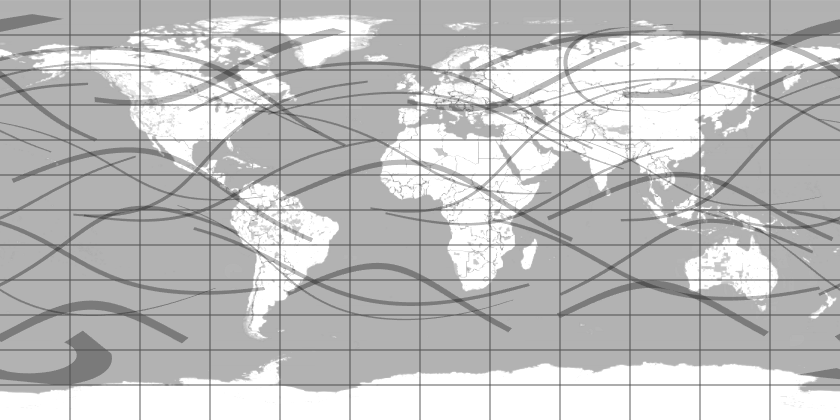
\includegraphics[width=\tw]{eclipses-map-20.png}
        \caption{Карта полных фаз затмений в 20-ом веке}
        \label{pic:eclipse-20-century}
    \end{subcaptionblock}
    \hfill
    \begin{subcaptionblock}[t]{0.32\tw}
        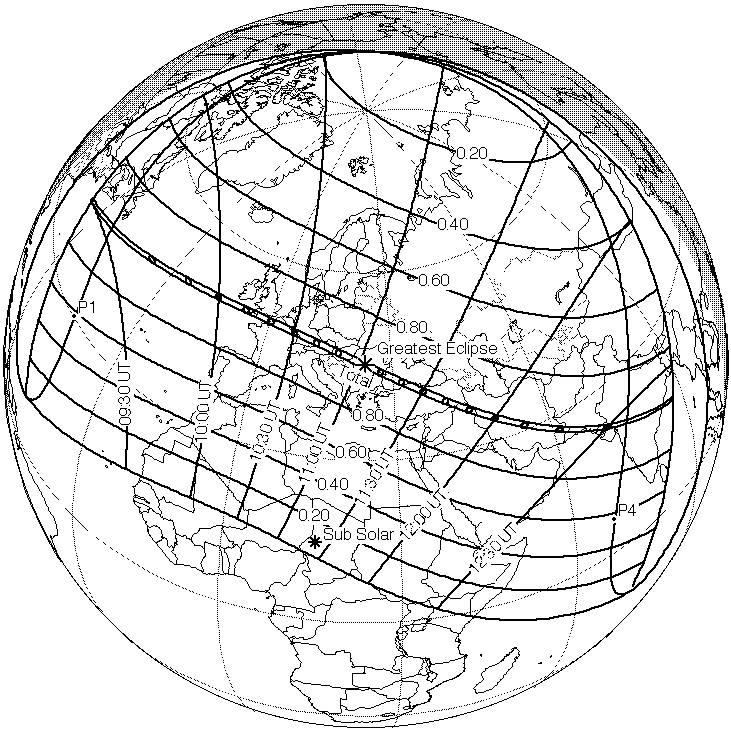
\includegraphics[width=\tw]{eclipse-map-1999-08-11.png}
        \caption{Карта затмения 11 августа 1999 года%\footnote{https://eclipse.gsfc.nasa.gov/SEplot/SEplot1951/SE1999Aug11T.GIF}
        }
        \label{pic:eclipse-1999-08-11}
    \end{subcaptionblock}
    \caption{}
\end{figure}

\begin{figure}[h!]
    \centering
    \vspace{-.5pc}
    \tikzsetnextfilename{eclipses-full-solar-eslipse}
    \begin{tikzpicture}
        \def\e{0}
        \def\m{-1.6}
        \def\s{-7.2}
        
        \def\earthR{0.7}
        \def\moonR{0.18}
        \def\sunR{1}
        
        \def\gap{0.2}
        
        \tkzInit[
            xmax=\e + \earthR + \gap,
            xmin=\s - \sunR - \gap,
            ymin=-\sunR - \gap,
            ymax=\sunR + \gap
        ]
        \tkzClip
        
        \tkzDefPoint(\e,0){E}
        \tkzDefPoint(\m,0){M}
        \tkzDefPoint(\s,0){S}
        
        \tkzDefShiftPoint[S](0,\sunR){S'}
        \tkzDefShiftPoint[M](0,\moonR){M'}
        \tkzDefShiftPoint[E](0,\earthR){E'}
        
        \def\shadeCornerCoef{\sunR / (\sunR - \moonR)}
        \tkzDefPointBy[homothety=center S ratio \shadeCornerCoef](M)
        \tkzGetPoint{SC}
        
        \def\halfShadowCornerCoef{\sunR / (\sunR + \moonR)}
        \tkzDefPointBy[homothety=center S ratio \halfShadowCornerCoef](M)
        \tkzGetPoint{HSC}
        
        \tkzDefLine[tangent from = SC](S,S')  \tkzGetPoints{S1}{S2}
        \tkzDefLine[tangent from = SC](M,M')  \tkzGetPoints{M1}{M2}
        \tkzDefLine[tangent from = HSC](S,S')  \tkzGetPoints{HS1}{HS2}
        \tkzDefLine[tangent from = HSC](M,M')  \tkzGetPoints{HM1}{HM2}
        
        \tkzInterLC(SC,S1)(E,E') \tkzGetSecondPoint{E1}
        \tkzInterLC(SC,S2)(E,E') \tkzGetFirstPoint{E2}
        
        \tkzGetVectxy(HSC,M){hs}
        \def\halfShadowCoef{(\e - \m + \hsx) / \hsx }
        \tkzDefPointBy[homothety=center HSC ratio \halfShadowCoef](HM1)
        \tkzGetPoint{HE1}
        \tkzDefPointBy[homothety=center HSC ratio \halfShadowCoef](HM2)
        \tkzGetPoint{HE2}
        
        \tkzDrawSector[fill=gray!30,gray!30](HSC,HE2)(HE1)
        \tkzDrawSector[fill=gray!70](SC,M2)(M1)
        \tkzDrawSector[fill=white](HSC,HM2)(HM1)
        
        \tkzDrawCircles[dashed, line width=.4pt](S,E E,M) 

        \tkzDrawCircles[black, line width=.4pt, fill=white](S,S' M,M')
        \tkzDrawSegments(SC,S1 SC,S2 HS1,HE1 HS2,HE2)
        
        \tkzDrawCircles[black, line width=.4pt, fill=white, fill opacity=1](E,E')
        
        \tkzLabelPoint[inner sep=5mm](S){\tikz{\sun(S)}}
        \tkzLabelPoint(E){\tikz{\earth(E)}}
        \tkzLabelPoint(M){$\rightmoon$}
    \end{tikzpicture}
    \caption{Полное солнечное затмение со стороны северного полюса эклиптики}
    \label{fig:eclipses-full-solar-eslipse}
\end{figure}
При \term[кольцеобразное солнечное затмение]{кольцеобразном солнечном затмении} Луна так расположена относительно Земли, что конус её тени не достаёт до поверхности планеты, и вокруг Луны можно наблюдать яркое кольцо незакрытой части солнечного диска.

\begin{figure}[h!]
    \centering
    \tikzsetnextfilename{eclipses-circle-solar-eslipse}
    \begin{tikzpicture}
        \def\e{0}
        \def\m{-2.2}
        \def\s{-7.2}
        
        \def\earthR{0.7}
        \def\moonR{0.18}
        \def\sunR{1}
        
        \def\gap{0.2}
        
        \tkzInit[
            xmax=\e + \earthR + \gap,
            xmin=\s - \sunR - \gap,
            ymin=-\sunR - \gap,
            ymax=\sunR + \gap
        ]
        \tkzClip
        
        \tkzDefPoint(\e,0){E}
        \tkzDefPoint(\m,0){M}
        \tkzDefPoint(\s,0){S}
        
        \tkzDefShiftPoint[S](0,\sunR){S'}
        \tkzDefShiftPoint[M](0,\moonR){M'}
        \tkzDefShiftPoint[E](0,\earthR){E'}
        
        \def\shadeCornerCoef{\sunR / (\sunR - \moonR)}
        \tkzDefPointBy[homothety=center S ratio \shadeCornerCoef](M)
        \tkzGetPoint{SC}
        
        \def\halfShadowCornerCoef{\sunR / (\sunR + \moonR)}
        \tkzDefPointBy[homothety=center S ratio \halfShadowCornerCoef](M)
        \tkzGetPoint{HSC}
        
        \tkzDefLine[tangent from = SC](S,S')  \tkzGetPoints{S1}{S2}
        \tkzDefLine[tangent from = SC](M,M')  \tkzGetPoints{M1}{M2}
        \tkzDefLine[tangent from = HSC](S,S')  \tkzGetPoints{HS1}{HS2}
        \tkzDefLine[tangent from = HSC](M,M')  \tkzGetPoints{HM1}{HM2}
        
        \tkzInterLC(SC,S1)(E,E') \tkzGetSecondPoint{E1}
        \tkzInterLC(SC,S2)(E,E') \tkzGetFirstPoint{E2}
        
        \tkzGetVectxy(HSC,M){hs}
        \def\halfShadowCoef{(\e - \m + \hsx) / \hsx }
        \tkzDefPointBy[homothety=center HSC ratio \halfShadowCoef](HM1)
        \tkzGetPoint{HE1}
        \tkzDefPointBy[homothety=center HSC ratio \halfShadowCoef](HM2)
        \tkzGetPoint{HE2}
        
        \tkzDefPointBy[homothety=center SC ratio -1](M1) \tkzGetPoint{SC1}
        \tkzDefPointBy[homothety=center SC ratio -1](M2) \tkzGetPoint{SC2}
        
        \tkzDrawSector[fill=gray!30,gray!30](HSC,HE2)(HE1)
        \tkzDrawSector[fill=gray!70](SC,M2)(M1)
        \tkzDrawSector[fill=gray!50](SC,SC2)(SC1)
        \tkzDrawSector[fill=white](HSC,HM2)(HM1)

        \tkzDrawCircles[dashed, line width=.4pt](S,E E,M) 

        \tkzDrawCircles[black, line width=.4pt, fill=white](S,S' M,M')
        \tkzDrawSegments(SC,S1 SC,S2 HS1,HE1 HS2,HE2)
        
        \tkzDrawCircles[black, line width=.4pt, fill=white, fill opacity=1](E,E')
        
        \tkzLabelPoint[inner sep=5mm](S){\tikz{\sun(S)}}
        \tkzLabelPoint(E){\tikz{\earth(E)}}
        \tkzLabelPoint(M){$\rightmoon$}
    \end{tikzpicture}
    \caption{Кольцеобразное солнечное затмение со стороны северного полюса эклиптики}
    \label{fig:eclipses-circle-solar-eslipse}
\end{figure}
При особом расположении Луны и Земли возможны \term{гибридные} затмения, когда в разных пунктах Земли наблюдаются либо \imp{кольцеобразное}, либо \imp{полное} затмение. Причиной такого явления является шарообразность Земли.

\vspace{-1pc}
\begin{figure}[h!]
    \centering
    \tikzsetnextfilename{moon-eclipse-scheme}
    \begin{tikzpicture}
        \def\e{2.2}
        \def\m{0}
        \def\s{-7.2}
        
        \def\earthR{0.25}
        \def\moonR{0.7}
        \def\sunR{1}
        
        \def\gap{0.2}
        
        \tkzInit[
            xmax=\e + \earthR + \gap,
            xmin=\s - \sunR - \gap,
            ymin=-\sunR - \gap,
            ymax=\sunR + \gap
        ]
        \tkzClip
        
        \tkzDefPoint(\e,0){E}
        \tkzDefPoint(\m,0){M}
        \tkzDefPoint(\s,0){S}
        
        \tkzDefShiftPoint[S](0,\sunR){S'}
        \tkzDefShiftPoint[M](0,\moonR){M'}
        \tkzDefShiftPoint[E](0,\earthR){E'}
        
        \def\shadeCornerCoef{\sunR / (\sunR - \moonR)}
        \tkzDefPointBy[homothety=center S ratio \shadeCornerCoef](M)
        \tkzGetPoint{SC}
        
        \def\halfShadowCornerCoef{\sunR / (\sunR + \moonR)}
        \tkzDefPointBy[homothety=center S ratio \halfShadowCornerCoef](M)
        \tkzGetPoint{HSC}
        
        \tkzDefLine[tangent from = SC](S,S')  \tkzGetPoints{S1}{S2}
        \tkzDefLine[tangent from = SC](M,M')  \tkzGetPoints{M1}{M2}
        \tkzDefLine[tangent from = HSC](S,S')  \tkzGetPoints{HS1}{HS2}
        \tkzDefLine[tangent from = HSC](M,M')  \tkzGetPoints{HM1}{HM2}
        
        \tkzGetVectxy(HSC,M){hs}
        \def\halfShadowCoef{1 + (\e - \m + \hsx) / \hsx }
        \tkzDefPointBy[homothety=center HSC ratio \halfShadowCoef](HM1)
        \tkzGetPoint{HE1}
        \tkzDefPointBy[homothety=center HSC ratio \halfShadowCoef](HM2)
        \tkzGetPoint{HE2}
        
        \tkzDrawSector[fill=gray!30,gray!30](HSC,HE2)(HE1)
        \tkzDrawSector[fill=gray!70](SC,M2)(M1)
        \tkzDrawSector[fill=white](HSC,HM2)(HM1)
        
        \tkzDrawCircles[dashed, line width=.4pt](S,M M,E)

        \tkzDrawCircles[black, line width=.4pt, fill=white](S,S' M,M')
        \tkzDrawSegments(SC,S1 SC,S2 HS1,HE1 HS2,HE2)
        
        \tkzDrawCircles[black, line width=.4pt, fill=white, fill opacity=1](E,E')
        
        \tkzLabelPoint[inner sep=5mm](S){\tikz{\sun(S)}}
        \tkzLabelPoint(M){\tikz{\earth(E)}}
        \tkzLabelPoint(E){$\rightmoon$}
    \end{tikzpicture}
    \caption{Схема лунного затмения со стороны северного полюса эклиптики}
    \label{fig:moon-eclipse-scheme}
\end{figure}
\term{Лунное затмение}, в отличие от солнечного, видно со всего ночного полушария Земли. Диаметр земной тени на расстоянии Луны превышает размер последней примерно в 2.5\,--\,3 раза. Бывают \term[частное затмение]{частные}, когда лишь часть Луны попадает в земную тень, \term[полное затмение]{полные}~--- Луна полностью погружается в тень Земли, и \term[полутеневое затмение]{полутеневые}~--- Луна проходит через полутень Земли, не затрагивая конус тени.

\begin{figure}[h!]
    \centering
    \tikzsetnextfilename{eclipses-full-lunar-eclipse}
    \begin{tikzpicture}
        \footnotesize
        
        % Radius of the Sun
        \def\RS{1.5}
        
        % Radius of the Earth
        \def\RE{1}
        
        % Radius of the Moon
        \def\RM{0.4}
    
        % Earth orbit radius
        \def\AE{3}
        
        % Moon orbit radius
        \def\AM{1.7}
        
        % ALPHA
        \pgfmathsetmacro\ALPHA{asin((\RS - \RE) / \AE)}
   
        % BETA
        \pgfmathsetmacro\BETA{acos((\RE - \RM) / \AM)}
     
        % GAMMA
        \pgfmathsetmacro\GAMMA{90 - \ALPHA - \BETA}
        
        % Earth
        \tkzDefPoint(0,0){E}
        \tkzDefCircle[R](E,\RE) \tkzGetPoint{e}
        
        % Sun
        \tkzDefShiftPoint[E](-\AE,0){S}
        \tkzDefCircle[R](S,\RS) \tkzGetPoint{s}
        
        % Moon
        \tkzDefShiftPoint[E](\AM,0){m}
        \tkzDefPointBy[rotation=center E angle \GAMMA](m) \tkzGetPoint{M}
        \tkzDefCircle[R](M,\RM) \tkzGetPoint{m}
        
        % Intersection of Sun-Earth and common tangent to Sun and Earth
        \tkzDefPointBy[homothety=center S ratio (\RS / (\RS - \RE))](E)
        \tkzGetPoint{I}

        % Tangent points of the Sun
        \tkzDefLine[tangent from = I](S,s) \tkzGetPoints{S'}{x}
        \tkzDefPointBy[reflection = over S--E](S') \tkzGetPoint{S''}

        % Tangent points of the Earth
        \tkzDefLine[tangent from = I](E,e) \tkzGetPoints{E'}{x}
        \tkzDefPointBy[reflection = over S--E](E') \tkzGetPoint{E''}
 
        % Tangent point of the Moon
        \tkzDefLine[tangent from = I](M,m) \tkzGetPoints{x}{M'}

        % Projection of the center of the Moon to the radius of the Earth
        \tkzDefPointBy[projection=onto E--E''](M) \tkzGetPoint{I'}
        
        % Intersection of a normal to Sun-Earth at the center of the Earth with common tangent of Sun and Earth
        \tkzDefPointWith[orthogonal,K=-1](E,I) \tkzGetPoint{x}
        \tkzInterLL(E,x)(I,E'') \tkzGetPoint{I''}

        % Draw shadow
        \tkzDrawPolygon[fill=gray!70,draw=none](E',I,E'')    
            
        % Draw objects
        \tkzDrawCircles[black, thick, fill=white](E,e)
        \tkzDrawCircles[black, thick, fill=white](S,s)
        \tkzDrawCircles[black, thick, fill=white](M,m)
        
        \begin{scope}[
            dim style/.style={black, latex-latex, opacity=1},
            dim fence style/.style={black, opacity=1}
        ]
            \tkzDrawSegment[opacity=0, dim={$D$, -1.6cm, below=2pt}](S,E)
        \end{scope}
        
        \tkzDrawSegments(S,I E,M S,S' S,S'' E,E' E,E'' M,M' E,I'')
        \tkzDrawSegments[semithick](S',I S'',I)
        \tkzDrawSegments[dashed](M,I')

        \tkzMarkRightAngles[size=0.15](I,E',E E,E'',I I,S',S S,S'',I I'',E,S E'',M',M E,I',M)

        \tkzMarkAngle[arc=l, size=0.7](E'',E,I'')
        \tkzMarkAngle[arc=l, size=1.3](E'',I,E)
        \tkzLabelAngle[pos=1.5](E'',I,E){\footnotesize$\alpha$}

        \tkzMarkAngle[arc=ll, size=0.25](M,E,I')
        \tkzLabelAngle[pos=0.5](M,E,I'){\footnotesize$\beta$}

        \tkzMarkAngle[arc=lll, size=1.5](I,E,M)
        \tkzLabelAngle[pos=1.7](I,E,M){\footnotesize$\gamma$}
        
        \tkzDrawPoints(S, S', S'')
        \tkzDrawPoints(E, E', E'')
        \tkzDrawPoints(M, M')
        \tkzDrawPoints(I, I', I'')
        
        \tkzLabelSegment[right](S,S'){$R_0$}
        \tkzLabelSegment[right](E,E'){$R$}
        \tkzLabelSegment[right=-1pt,pos=0.4](M,M'){$r$}
        \tkzLabelSegment[above=-1pt,pos=0.45](E,M){$d$}
    \end{tikzpicture}
    \caption{}
    \label{pic:eclipses-full-lunar-eslipse}
\end{figure}

\begin{figure}[h!]
    \centering
    \tikzsetnextfilename{eclipses-semi-shadow-lunar-eclipse}
    \begin{tikzpicture}
        \footnotesize
        
        % Radius of the Sun
        \def\RS{1.4}
        
        % Radius of the Earth
        \def\RE{0.9}
        
        % Radius of the Moon
        \def\RM{0.4}
    
        % Earth orbit radius
        \def\AE{5}
        
        % Moon orbit radius
        \def\AM{2}
        
        \tkzInit[
            xmax=3.0,
            xmin=-6.5,
            ymin=-2.2,
            ymax=2.2
        ]
        
        \tkzClip
        
        % ALPHA
        \pgfmathsetmacro\ALPHA{asin((\RS + \RE) / \AE)}
   
        % BETA
        \pgfmathsetmacro\BETA{acos((\RE - \RM) / \AM)}
     
        % GAMMA
        \pgfmathsetmacro\GAMMA{90 + \ALPHA - \BETA}
        
        % Earth
        \tkzDefPoint(0,0){E}
        \tkzDefCircle[R](E,\RE) \tkzGetPoint{e}
        
        % Sun
        \tkzDefShiftPoint[E](-\AE,0){S}
        \tkzDefCircle[R](S,\RS) \tkzGetPoint{s}
        
        % Moon
        \tkzDefShiftPoint[E](\AM,0){m}
        \tkzDefPointBy[rotation=center E angle \GAMMA](m) \tkzGetPoint{M}
        \tkzDefCircle[R](M,\RM) \tkzGetPoint{m}
        
        % Intersections of Sun-Earth and common tangent to Sun and Earth
        \tkzDefPointBy[homothety=center S ratio (\RS / (\RS - \RE))](E)
        \tkzGetPoint{I}
        \tkzDefPointBy[homothety=center S ratio (\RS / (\RS + \RE))](E)
        \tkzGetPoint{I'}
        
        % Full shadow tangent points of the Sun
        \tkzDefLine[tangent from = I](S,s) \tkzGetPoints{S'}{x}
        \tkzDefPointBy[reflection = over S--E](S') \tkzGetPoint{S''}
        
        % Semi-shadow tangent points of the Sun
        \tkzDefLine[tangent from = I'](S,s) \tkzGetPoints{SsS'}{x}
        \tkzDefPointBy[reflection = over S--E](SsS') \tkzGetPoint{SsS''}

        % Full shadow tangent points of the Earth
        \tkzDefLine[tangent from = I](E,e) \tkzGetPoints{E'}{x}
        \tkzDefPointBy[reflection = over S--E](E') \tkzGetPoint{E''}
        
        % Semi-shadow tangent points of the Earth
        \tkzDefLine[tangent from = I'](E,e) \tkzGetPoints{SsE'}{x}
        \tkzDefPointBy[reflection = over S--E](SsE') \tkzGetPoint{SsE''}
 
        % Tangent point of the Moon
        \tkzDefLine[tangent from = I'](M,m) \tkzGetPoints{M'}{x}
        
        % Projection of the center of the Moon to the radius of the Earth
        \tkzDefPointBy[projection=onto E--SsE'](M) \tkzGetPoint{I''}
        
        % Semishadow
        \tkzDefPointBy[homothety=center SsE'' ratio -1.7](I') \tkzGetPoint{Ss1}
        \tkzDefPointBy[homothety=center SsE' ratio -1.7](I') \tkzGetPoint{Ss2}
        
        % Draw semishadow
        \tkzFillSector[gray!30](I',Ss1)(Ss2)
        \tkzFillSector[white](I',SsE'')(SsE')
        \tkzDrawSegments[semithick](SsS',Ss2 SsS'',Ss1)  

        % Draw shadow
        \tkzDrawPolygon[fill=gray!70,draw=none](E',I,E'') 
            
        % Draw objects
        \tkzDrawCircles[black, thick, fill=white](E,e)
        \tkzDrawCircles[black, thick, fill=white](S,s)
        \tkzDrawCircles[black, thick, fill=white](M,m)
        
        \begin{scope}[
            dim style/.style={black, latex-latex, opacity=1},
            dim fence style/.style={black, opacity=1}
        ]
            \tkzDrawSegment[opacity=0, dim={$D$, -1.6cm, below=2pt}](S,E)
            \tkzDrawSegment[opacity=0, dim={$d$, 1.1cm, below right=1pt, pos=0.46, fill=none}](M,E)
        \end{scope}
        
        \tkzDrawSegments(S,I E,M S,S' S,S'' E,E' M,M' E,SsE' E,SsE'' S,SsS' S,SsS'')
        \tkzDrawSegments[semithick](S',I S'',I)
        \tkzDrawSegments[dashed](M,I'')

        \tkzMarkRightAngles[size=0.15](I,E',E I,S',S S,S'',I SsE',M',M E,SsE',Ss2 S,SsS',I' I',SsS'',S Ss1,SsE'',E M,I'',SsE')
 
        \tkzMarkAngle[arc=l, size=0.5](E,I',SsE')
        \tkzLabelAngle[pos=0.7](E,I',SsE'){\footnotesize$\alpha$}
        
        \tkzMarkAngle[arc=ll, size=0.2](M,E,SsE')
        \tkzLabelAngle[pos=0.4](M,E,SsE'){\footnotesize$\beta$}

        \tkzMarkAngle[arc=lll, size=0.4](I,E,M)
        \tkzLabelAngle[pos=0.6](I,E,M){\footnotesize$\gamma$}
        
        \tkzDrawPoints(S, S', S'', SsS', SsS'')
        \tkzDrawPoints(E, E', E'', SsE', SsE'')
        \tkzDrawPoints(M, M')
        \tkzDrawPoints(I, I')
        
        \tkzLabelSegment[left](S,S''){$R_0$}
        \tkzLabelSegment[left](E,SsE'){$R$}
        \tkzLabelSegment[right=-1pt,pos=0.4](M,M'){$r$}
    \end{tikzpicture}
    \caption{}
    \label{pic:eclipses-semi-shadow-lunar-eclipse}    
\end{figure}


\term{Синодический месяц}~--- промежуток времени между одинаковыми фазами Луны, равен 29.53 суток.

\term{Драконический месяц}~--- промежуток времени между двумя последовательными прохождениями Луны через один и тот же узел орбиты,~--- 27.21 суток.

\term{Сарос}~--- промежуток  времени, по прошествии которого солнечные и лунные затмения повторяются в прежнем порядке. Происходит это из-за того, что каждый сарос Луна, орбита Луны и Солнце возвращаются в прежнее положение относительно далёких звёзд. Сарос длится ровно 242 драконических месяца, или 223 синодических месяца, или 18 лет 11 дней 8 часов.

\begin{wrapfigure}[15]{r}{.27\tw}
    \centering
    \vspace{-1pc}
    \begin{subcaptionblock}[t]{.27\tw}
        \centering
        \tikzsetnextfilename{part-eclipses-scheme1}
        \begin{tikzpicture}
            \tkzDefPoint(0,0){C1}
            \tkzDefPoint(-0.6,0.6){C2}

            \def\R{0.7}
            \def\r{0.6}

            \tkzDefShiftPoint[C2](\r,0){R2}
            \tkzDrawCircle[semithick, draw=black, fill=white](C2,R2)

            \tkzDefShiftPoint[C1](\R,0){R1}
            \tkzDrawCircle[semithick, draw=black, fill=black!30](C1,R1)

            \tkzInterCC(C1,R1)(C2,R2) \tkzGetPoints{I1}{I2}
            \tkzInterLC(C1,C2)(C1,R1) \tkzGetPoints{x}{L1}
            \tkzInterLC(C1,C2)(C2,R2) \tkzGetPoints{L2}{x}

            \tkzDrawArc[semithick, dashed](C2,I1)(I2)

            \tkzDrawSegment(C1,C2)
            \tkzDrawSegment[latex-latex](L1,L2)

            \tkzDefPointBy[homothety=center C2 ratio -1](R2) \tkzGetPoint{R2'}

            \tkzDrawSegment[
                dim style/.append style={opacity=1},
                dim fence style/.style={opacity=1},
                dim={$D$, \fpeval{\r + 0.1} cm, above=2pt},
                opacity=0
            ](R2',R2)

            \tkzLabelSegment[above right=-2pt](L1,L2){$x$}

            \tkzDrawPoints(C1, C2)
        \end{tikzpicture}
        \caption{Частное}
        \label{pic:partial-esclipse-phase}
    \end{subcaptionblock}
    \begin{subcaptionblock}[t]{.27\tw}
        \centering
        \tikzsetnextfilename{part-eclipses-scheme2}
        \begin{tikzpicture}
            \tkzDefPoint(0,0){C1}
            \tkzDefPoint(-0.2,-0.2){C2}

            \def\R{1.3}
            \def\r{0.6}

            \tkzDefShiftPoint[C1](\R,0){R1}
            \tkzDrawCircle[semithick, draw=black, fill=black!30](C1,R1)

            \tkzDefShiftPoint[C2](\r,0){R2}
            \tkzDrawCircle[semithick, draw=black, dashed](C2,R2)

            \tkzInterLC(C1,C2)(C1,R1) \tkzGetPoints{L1}{L2}
            \tkzInterLC(C1,C2)(C2,R2) \tkzGetPoints{I1}{I2}

            \tkzDefPointBy[homothety=center C2 ratio -1](R2) \tkzGetPoint{R2'}

            \tkzDrawSegment(L1,L2)
            \tkzDrawSegments[latex-latex](L1,I1 L2,I2)

            \tkzDrawSegment[
                dim style/.append style={opacity=1},
                dim fence style/.style={opacity=1},
                dim={$D$, \fpeval{\r + 0.1} cm, above=2pt, fill=none},
                opacity=0
            ](R2',R2)

            \tkzLabelSegment[below right=-4pt](L1,I1){$d_1$}
            \tkzLabelSegment[below right=-4pt](L2,I2){$d_2$}

            \tkzDrawPoints(C1, C2)
        \end{tikzpicture}
        \caption{Полное}
        \label{pic:full-esclipse-phase}
    \end{subcaptionblock}
    \caption{Схемы затмений}
    \label{fig:part-eclipses-scheme}
\end{wrapfigure}
Важной характеристикой любого затмения является его \term{фаза}~--- для \imp{частных} и \imp{кольцеобразных} затмений: отношение закрытой части $x$ диаметра\footnote{Здесь имеется в виду \imp{угловой} диаметр} затмеваемого тела, проходящего через центр затмевающего тела, ко всему диаметру затмеваемого тела $D$; для \imp{полного}: единица плюс отношение расстояния\footnote{Расстояние между окружностями $l_1$ и $l_2$~--- это $\min |L_1L_2|$ по всем $L_1 \in l_1$ и $L_2 \in l_2$.} между краями дисков затмеваемого и затмевающего тел к диаметру затмеваемого тела $D$.
\begin{align}
    \Phi_{\text{част}} &= \frac{x}{D}< 1,\\
    \Phi_{\text{полн}} &= 1 + \frac{\min\{d_1, d_2\}}{D}> 1.
\end{align}
Иногда вводят такое понятие, как \term{площадная фаза затмения}, т.\,е. отношение площади закрытой части диска затмеваемого тела к полной площади его диска. Чаще всего площадную фазу используют применительно к двойным звёздам, когда считают падение блеска при затмении одной звезды другой.
